%! Author = Antonio Lobo
%! Date = 30/10/2024

\section{Reduction Methods}
In this section we will briefly describe the reductions techniques employed for instance based learning. We will use a simple 2D dataset ($D_1$) for illustrations purposes that can be seen in \textbf{Figure} \ref{fig:2dDatasetReduction}.
\begin{figure}[ht]
    \centering
    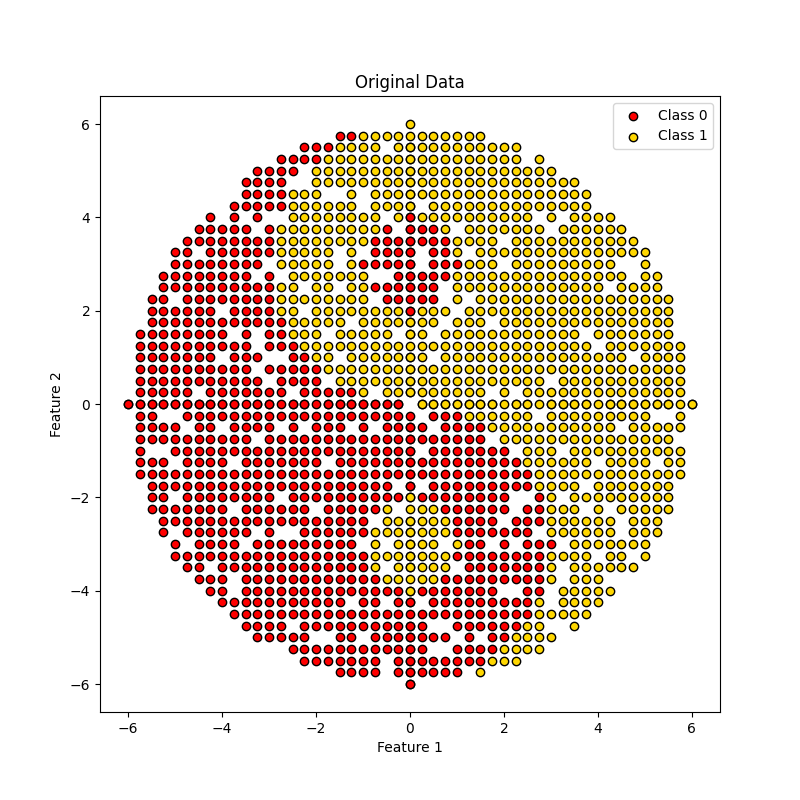
\includegraphics[width=\textwidth]{figures/2dDataset} % Adjust the path and size as needed
    \caption{2D example dataset}
    \label{fig:2dDatasetReduction}
\end{figure}


\subsection{DROP3}:
In this subsection we will describe the basics concepts of the third method of the family Decremental Reduction Optimization Procedure (DROP) which can be found in the third section of Wilson et al \cite{wilson2000reduction}.
Although we will not go into the details we will like to describe the idea of the algorithm with a simple example in 2D that have been generated for illustration purposes and that can be seen in :

\begin{enumerate}
    \item \textbf{Remove noise}: The first step is to remove noisy instances using EEN \cite{wilson1972asymptotic} where any instance misclassified by its k nearest neighbors is removed. The result of applying this technique can be seen in \textbf{Figure} \ref{fig:2dEEN} where we can easily seen that noise have been removed.
    \begin{figure}[ht]
        \centering
        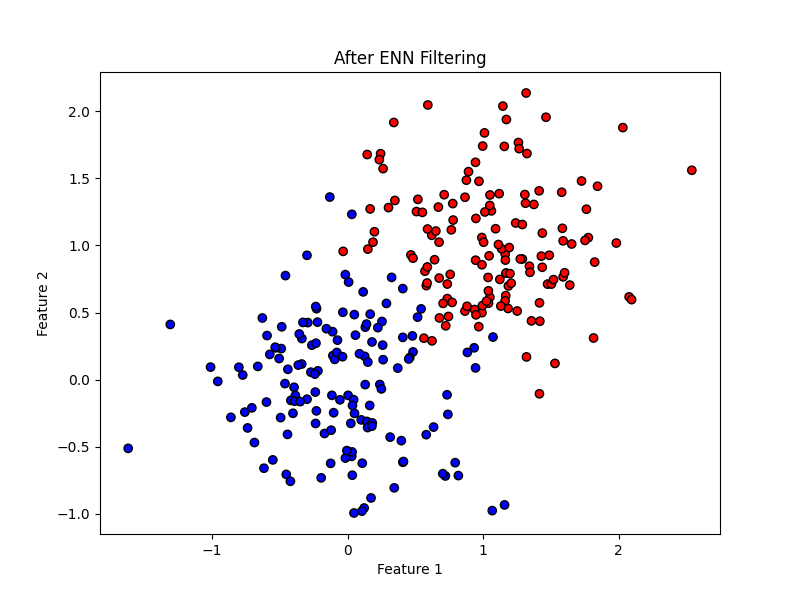
\includegraphics[width=\textwidth]{figures/2dEEN} % Adjust the path and size as needed
        \caption{Example of EEN noise removal}
        \label{fig:2dEEN}
    \end{figure}
\end{enumerate}

